% !TEX program = pdflatex
% ============================================================================
% Problem Set 1 - Section 3: Income Prediction
% Slide deck. Every number, table and figure is pulled from output/ so the
% deck stays in sync with script/06_income_prediction_train.r,
% script/07_income_prediction_validation.r and
% script/08_income_imputation_comparison.r: re-run those three scripts (in
% order), recompile this file, done. Nothing is hard-coded here.
%
%   - \input ../../output/tables/section3_prediction_stats.tex          (numbers as macros)
%   - \input ../../output/tables/section3_imputation_stats.tex          (numbers as macros)
%   - \input ../../output/tables/section3_model_comparison_slide.tex    (10-model table)
%   - \input ../../output/tables/section3_imputation_comparison_slide.tex (complete vs. imputed)
%   - ../../output/figures/section3_variable_importance.png            (standardized betas, best model)
%   - ../../output/figures/section3_imputation_density.png             (observed vs. imputed log-income)
%
% section3_subgroup_rmse.png (bias check by subgroup) is not used here - it
% has no slide of its own in this deck, kept out to hold the length down.
%
% Compile from inside presentation/:  pdflatex income_prediction_slides.tex
% Export/submit as pred_equipo_XX.pdf (XX = team number; see \teamnumber below).
% ============================================================================
\documentclass[aspectratio=169]{beamer}

\usepackage[utf8]{inputenc}
\usepackage[T1]{fontenc}
\usepackage[spanish,es-noshorthands]{babel}
\usepackage{booktabs}
\usepackage{graphicx}
\usepackage{amsmath}
\usepackage{xcolor}

% uandespurple: deck accent (frame titles, structure), same as
% age_income_slides.tex for visual continuity across the three decks.
% predblue/predpurple match the two fill colours used throughout the
% Section 3 figures (section3_variable_importance.png,
% section3_imputation_density.png), so in-slide highlights carry the same
% colour as the plots.
\definecolor{uandespurple}{HTML}{6C0A8A}
\definecolor{predblue}{HTML}{4DAAD5}
\definecolor{predpurple}{HTML}{6C0A8A}

\usetheme{Boadilla}
\setbeamercolor{structure}{fg=uandespurple}
\setbeamercolor{frametitle}{fg=uandespurple}
\setbeamercolor{title}{fg=uandespurple}
\setbeamertemplate{navigation symbols}{}
\setbeamertemplate{caption}[numbered]
\setbeamerfont{frametitle}{size=\large}

% Key numbers (best model, RMSE/AIC/BIC, imputation counts, ...) as LaTeX macros.
\newcommand{\PredNModels}{10}
\newcommand{\PredNTrain}{10,263}
\newcommand{\PredNValidation}{4,500}
\newcommand{\PredBestModel}{Gender: HK + hours (05)}
\newcommand{\PredBestValRMSE}{0.7451}
\newcommand{\PredBestLOOCV}{0.7204}
\newcommand{\PredBestAIC}{22,476}
\newcommand{\PredBestBIC}{22,555}
\newcommand{\PredSecondModel}{Formal x firm size x college}
\newcommand{\PredSecondValRMSE}{0.7452}

\newcommand{\ImpNComplete}{10,263}
\newcommand{\ImpNTotal}{11,382}
\newcommand{\ImpNImputed}{1,119}
\newcommand{\ImpMDraws}{5}
\newcommand{\ImpNRelabExcl}{165}


\newcommand{\teamnumber}{XX}

\title[Predicción del ingreso]{Predicción del ingreso laboral en Bogotá}
\subtitle{Problem Set 1 \textbullet\ Sección 3}
\author[Perez, Lozano, Suarez]{María José Pérez \and Juan Manuel Lozano \and Samuel Suárez Valle}
\institute[Uniandes]{MECA 4107 --- Big Data y Machine Learning para Economía Aplicada}
\date{Septiembre 2026}

\begin{document}

\begin{frame}[plain]
  \titlepage
\end{frame}

% ---------------------------------------------------------------------------
% Slide 1 (mandatory): Result Overview
% ---------------------------------------------------------------------------
\begin{frame}{Resultado principal}
  \begin{block}{Un modelo de la Sección 2 predice mejor que las cinco especificaciones nuevas}
    \begin{itemize}
      \item Comparamos \textbf{\PredNModels\ especificaciones} --- las 5 de las
        Secciones 1--2 más 5 nuevas --- entrenadas en \texttt{subset} 1--7
        (\PredNTrain\ obs.) y validadas en \texttt{subset} 8--10
        (\PredNValidation\ obs.), nunca vistos durante el ajuste.
      \item \textbf{Ganador:} \PredBestModel, con RMSE de validación
        \textbf{\PredBestValRMSE} (escala $\log$ ingreso), LOOCV
        \textbf{\PredBestLOOCV}, AIC \textbf{\PredBestAIC}, BIC \textbf{\PredBestBIC}.
      \item Le sigue muy de cerca \PredSecondModel\ (RMSE \PredSecondValRMSE)
        --- una de nuestras especificaciones nuevas, con la misma capacidad
        predictiva que el mejor modelo de la Sección 2.
      \item Los tres criterios (RMSE de validación, LOOCV, AIC/BIC) coinciden en
        el ranking: una señal de que la comparación es robusta, no un
        artefacto de un solo criterio.
    \end{itemize}
  \end{block}
  \vfill
  {\footnotesize Todas las regresiones ponderadas por \texttt{fex\_c}. RMSE y
  LOOCV en escala $\log(\text{y\_total\_m})$.}
\end{frame}

% ---------------------------------------------------------------------------
\begin{frame}{Enfoque: validación con datos nunca vistos}
  \textbf{¿Qué especificación predice mejor el ingreso laboral de individuos que
  el modelo nunca observó?}
  \vspace{0.4em}
  \begin{itemize}
    \item La GEIH se raspó en 10 \emph{chunks}; usamos esa partición natural
      como split \textbf{entrenamiento (1--7) / validación (8--10)}, en vez de
      un split aleatorio.
    \item Cada una de las \PredNModels\ especificaciones se ajusta \textbf{solo}
      con el entrenamiento y se evalúa contra el ingreso \emph{real} observado
      en la validación --- nunca contra un valor que nosotros mismos generamos.
    \item Este es el criterio más exigente: un modelo puede ajustar muy bien
      dentro de muestra ($R^2$ alto) y aun así predecir mal en datos nuevos si
      sobreajusta.
  \end{itemize}
\end{frame}

% ---------------------------------------------------------------------------
\begin{frame}{Cómo comparamos: cuatro criterios, no uno}
  \begin{columns}[T]
    \begin{column}{0.5\textwidth}
      \textbf{Fuera de muestra}
      \begin{itemize}
        \item \textbf{RMSE de validación}: error de predicción sobre el
          \texttt{subset} 8--10, nunca usado para ajustar. El criterio que
          pide el problem set.
        \item \textbf{LOOCV vía \emph{leverage}}: en vez de reajustar cada
          modelo $n$ veces, usamos el atajo exacto de mínimos cuadrados
          \[e_{(i)} = \frac{e_i}{1-h_{ii}}\]
          con $h_{ii}$ el \emph{leverage} de la observación $i$ --- un solo
          ajuste reproduce el resultado de $n$ regresiones leave-one-out.
      \end{itemize}
    \end{column}
    \begin{column}{0.5\textwidth}
      \textbf{Dentro de muestra}
      \begin{itemize}
        \item \textbf{AIC / BIC}: ajuste penalizado por número de parámetros
          (BIC penaliza más fuerte); complementan el RMSE con una medida de
          parsimonia.
        \item[]
        \item \textcolor{predpurple}{\textbf{Advertencia:}} AIC/BIC solo son
          comparables entre modelos ajustados sobre \emph{el mismo} $n$. Por
          eso, en la comparación completos-vs-imputado (más adelante) solo
          usamos RMSE de validación entre columnas.
      \end{itemize}
    \end{column}
  \end{columns}
\end{frame}

% ---------------------------------------------------------------------------
\begin{frame}{Diez especificaciones}
  \begin{columns}[T]
    \begin{column}{0.48\textwidth}
      \textbf{Secciones 1--2 (ya estimadas)}
      \begin{itemize}
        \footnotesize
        \item Edad: incondicional y condicional
        \item Género: incondicional, con capital humano, con capital humano + horas
      \end{itemize}
    \end{column}
    \begin{column}{0.48\textwidth}
      \textbf{Cinco especificaciones nuevas}
      \begin{itemize}
        \footnotesize
        \item Formalidad $\times$ tamaño de firma $\times$ college
        \item Subsidio familiar $\times$ college
        \item Cuenta propia $\times$ college
        \item Horas$^2$ $\times$ transferencias
        \item Género $\times$ nivel educativo
      \end{itemize}
    \end{column}
  \end{columns}
  \vspace{0.6em}
  \begin{itemize}
    \item Cada especificación nueva agrega una \textbf{no-linealidad o
      interacción} justificada por una hipótesis económica concreta y
      contrastada con literatura (siguientes dos diapositivas).
  \end{itemize}
\end{frame}

% ---------------------------------------------------------------------------
\begin{frame}{Especificaciones nuevas (I): formalidad y beneficios}
  \[
    \log(w_i) = \beta_1 + \beta_2\,\text{college}_i + \beta_3\,\text{formal}_i
      + \sum_k \gamma_k\,\text{sizeFirm}_{k,i} + \delta\,(\text{formal}_i \times \text{college}_i) + u_i
  \]
  \begin{itemize}
    \item \textbf{Formalidad $\times$ tamaño de firma $\times$ college:} los
      trabajos formales agrupan protecciones legales y acceso a empleadores
      más capitalizados; firmas grandes pagan más por el mismo trabajador
      (mercados laborales internos). La interacción prueba si el título
      universitario se premia más dentro del sector formal, donde el empleador
      puede verificarlo.
    \item \textbf{Subsidio familiar $\times$ college:} el subsidio familiar
      (cajas de compensación) es un beneficio no salarial atado a un empleo
      formal --- "buenos trabajos" agrupan mayor pago \emph{y} este tipo de
      beneficio.
  \end{itemize}
  \vfill
  {\footnotesize \textbf{Literatura:} Brown, C. \& Medoff, J. (1989). ``The
  Employer Size-Wage Effect.'' \emph{Journal of Political Economy}, 97(5),
  1027--1059 --- documenta que firmas grandes pagan más, en parte vía mejores
  beneficios no salariales, no solo salario base.}
\end{frame}

% ---------------------------------------------------------------------------
\begin{frame}{Especificaciones nuevas (II): autoempleo, horas y género}
  \begin{itemize}
    \item \textbf{Cuenta propia $\times$ college:} el cuentapropismo es, en
      promedio, una penalidad de ingreso (restricciones de liquidez, sin
      beneficios); pero el cuentapropismo profesional (independientes con
      título) es una población distinta de la de subsistencia.
      {\footnotesize Levine, R. \& Rubinstein, Y. (2017). ``Smart and Illicit:
      Who Becomes an Entrepreneur and Do They Earn More?'' \emph{QJE}, 132(2),
      963--1018.}
    \item \textbf{Horas$^2$ $\times$ transferencias:} retornos decrecientes a
      horas extra (jornadas asalariadas con tope), y el ingreso no laboral
      (transferencias) amortigua la intensidad de la oferta laboral.
      {\footnotesize Bick, A., Blandin, A. \& Rogerson, R. (2022). ``Hours and
      Wages.'' \emph{QJE}, 137(3), 1901--1962.}
    \item \textbf{Género $\times$ nivel educativo:} deja que cada nivel
      educativo tenga su propia brecha de género, en vez de un solo
      desplazamiento --- prueba si la brecha se \emph{ensancha} con las
      credenciales.
      {\footnotesize Goldin, C. (2014). ``A Grand Gender Convergence: Its Last
      Chapter.'' \emph{American Economic Review}, 104(4), 1091--1119.}
  \end{itemize}
\end{frame}

% ---------------------------------------------------------------------------
\begin{frame}{Comparación de las diez especificaciones}
  \centering
  {\scriptsize 
\begin{tabular}[t]{lrrrr}
\toprule
Model & LOOCV RMSE & Val. RMSE & AIC & BIC\\
\midrule
Gender: HK + hours (05) & 0.720 & 0.745 & 22475.56 & 22555.15\\
Formal x firm size x college & 0.725 & 0.745 & 22608.85 & 22688.44\\
Género x nivel educativo & 0.763 & 0.776 & 23657.25 & 23765.80\\
Subsidio familiar x college & 0.749 & 0.779 & 23311.97 & 23406.04\\
Gender: HK controls (05) & 0.766 & 0.779 & 23735.73 & 23808.09\\
\addlinespace
Horas\textasciicircum{}2 x transferencias & 0.779 & 0.809 & 24087.85 & 24152.98\\
Age: conditional (04) & 0.779 & 0.812 & 24072.60 & 24152.20\\
Cuenta propia x college & 0.822 & 0.841 & 25177.06 & 25227.71\\
Age: unconditional (04) & 0.866 & 0.892 & 26267.86 & 26296.81\\
Gender: unconditional (05) & 0.881 & 0.907 & 26632.06 & 26653.77\\
\bottomrule
\end{tabular}
}

  \vspace{0.5em}
  {\footnotesize Ordenado por RMSE de validación. LOOCV vía atajo de
  \emph{leverage} (diapositiva anterior); AIC/BIC comparables entre estas diez
  filas porque todas se ajustan sobre el mismo \PredNTrain\ (mismo $n$).}
\end{frame}

% ---------------------------------------------------------------------------
\begin{frame}{¿Qué variables pesan más? Coeficientes estandarizados}
  \begin{columns}[T]
    \begin{column}{0.42\textwidth}
      \textbf{¿Por qué estandarizar?}
      \begin{itemize}
        \small
        \item El coeficiente crudo de \texttt{age} (años) y de una dummy 0/1
          no son comparables en magnitud: dependen de la escala de cada
          variable.
        \item $\beta^{std} = \beta \cdot \dfrac{sd(x)}{sd(y)}$ pone a todas
          las variables --- continuas, dummies, niveles de factor --- en la
          misma unidad: desviaciones estándar de $\log$ ingreso por
          desviación estándar de $x$.
        \item Así, ``importancia'' compara \emph{efecto económico}, no solo
          significancia estadística.
      \end{itemize}
    \end{column}
    \begin{column}{0.58\textwidth}
      \centering
      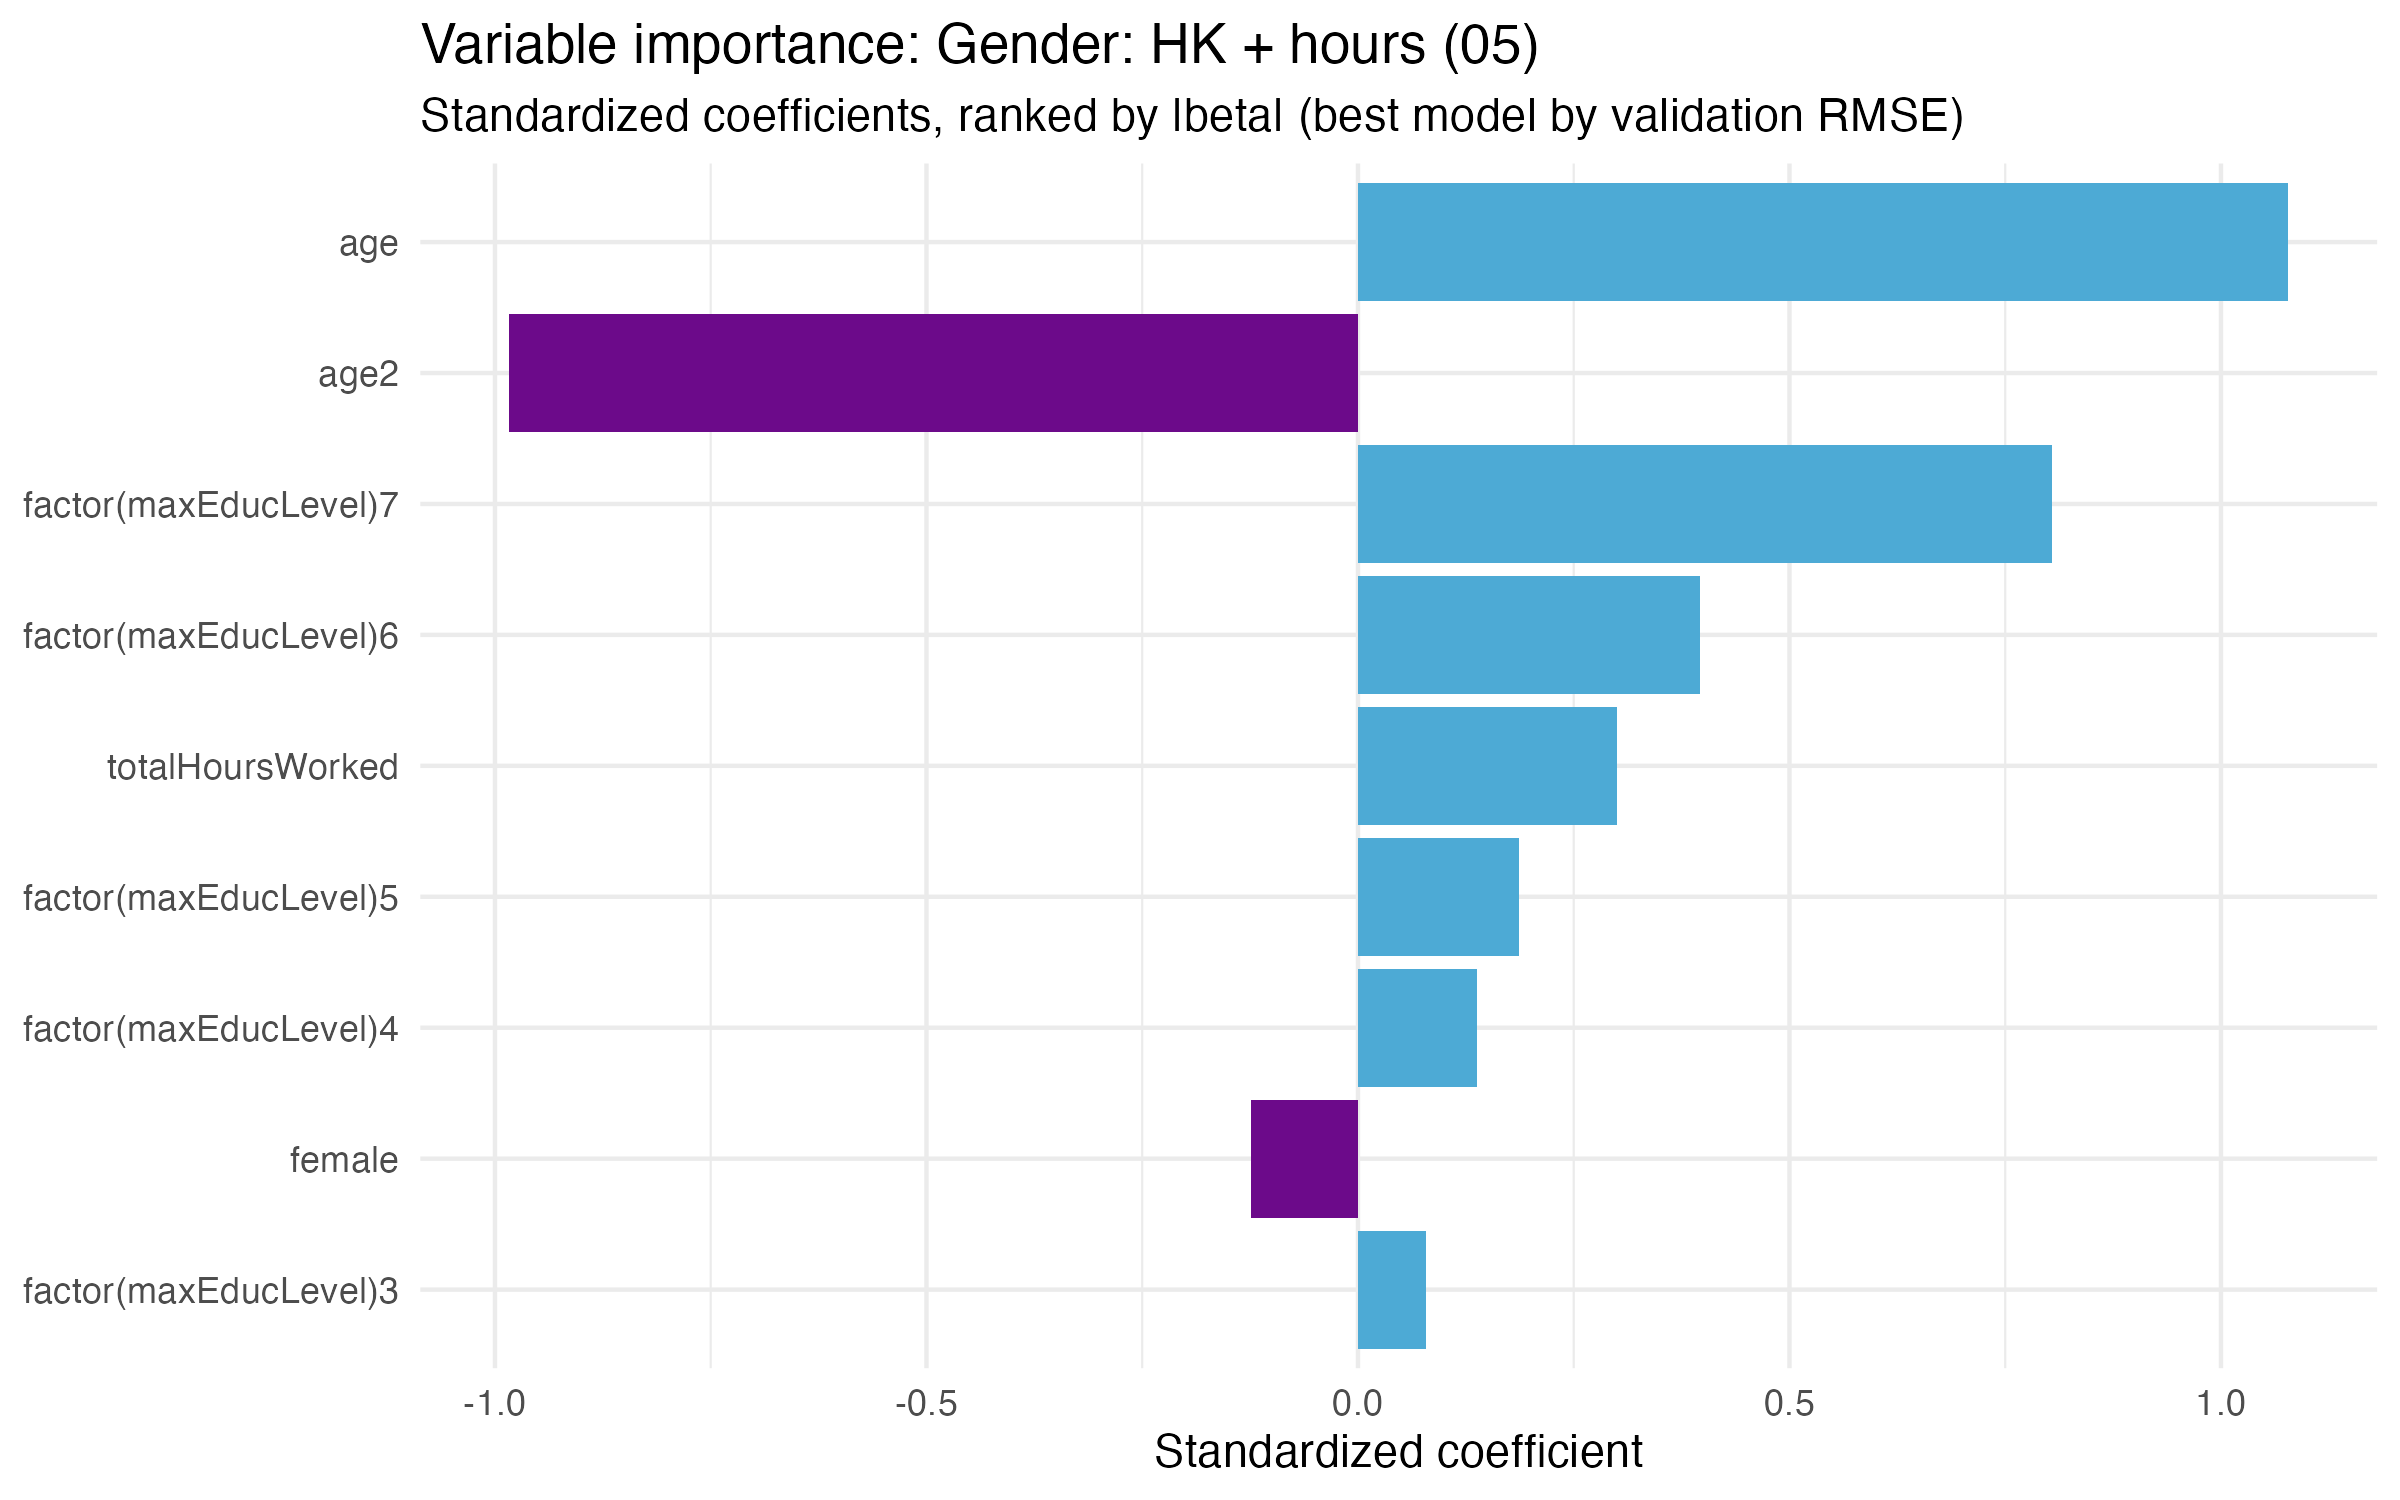
\includegraphics[width=\textwidth]{../../output/figures/section3_variable_importance.png}
    \end{column}
  \end{columns}
\end{frame}

% ---------------------------------------------------------------------------
\begin{frame}{El problema: el ingreso faltante no es aleatorio}
  \begin{itemize}
    \item La \emph{balance table} de \texttt{02\_data\_cleaning.r} mostró que
      \texttt{y\_total\_m} falta con más frecuencia entre trabajadores por
      cuenta propia, empleadores e informales --- y casi siempre entre
      trabajadores familiares sin remuneración (\texttt{relab} 6--7).
    \item Nuestro modelo, entrenado solo con \texttt{y\_total\_m > 0}, en la
      práctica \textbf{nunca aprende} de esa población: cada RMSE de
      validación mostrado hasta aquí describe qué tan bien predecimos a quien
      reporta ingreso, no a todos los ocupados.
    \item \textbf{Pregunta:} ¿ese sesgo de selección distorsiona el ranking de
      modelos, o el desempeño se sostiene si enriquecemos el entrenamiento?
    \item \texttt{relab} 6--7 (\ImpNRelabExcl\ obs.) se excluyen de este
      ejercicio: no tienen salario monetario por definición, no un dato
      faltante por corregir.
  \end{itemize}
\end{frame}

% ---------------------------------------------------------------------------
\begin{frame}{Metodología: imputación múltiple con MICE / PMM}
  \begin{itemize}
    \item \textbf{MICE} (\emph{Multivariate Imputation by Chained Equations}):
      genera $m$ bases de datos completas, cada una con un sorteo distinto
      para cada valor faltante --- así el análisis final puede reflejar la
      incertidumbre de la imputación en vez de fingir que el dato faltante
      ahora es "conocido con certeza".
    \item \textbf{PMM} (\emph{Predictive Mean Matching}), el método que usamos
      dentro de MICE:
      \begin{enumerate}
        \small
        \item Ajusta un modelo de $\log(\text{ingreso})$ con predictores
          completamente observados (edad, sexo, educación, \texttt{relab},
          formalidad, horas, tamaño de firma, cuenta propia).
        \item Para cada faltante, busca sus 5 vecinos más parecidos (por valor
          predicho) entre quienes sí reportan ingreso.
        \item Sortea \textbf{uno} de esos 5 vecinos y copia su ingreso
          \emph{observado} --- nunca un valor inventado por el modelo.
      \end{enumerate}
    \item Es el mismo principio que usan agencias oficiales (p.\ ej.\ el hot-deck
      de la CPS del US Census Bureau) para imputar ingreso faltante.
    \item Imputamos \ImpNImputed\ observaciones ($m = \ImpMDraws$ sorteos cada
      una), ampliando el entrenamiento de \ImpNComplete\ a \ImpNTotal\ filas.
  \end{itemize}
\end{frame}

% ---------------------------------------------------------------------------
\begin{frame}{Diagnóstico y resultado de la imputación}
  \begin{columns}[T]
    \begin{column}{0.48\textwidth}
      \centering
      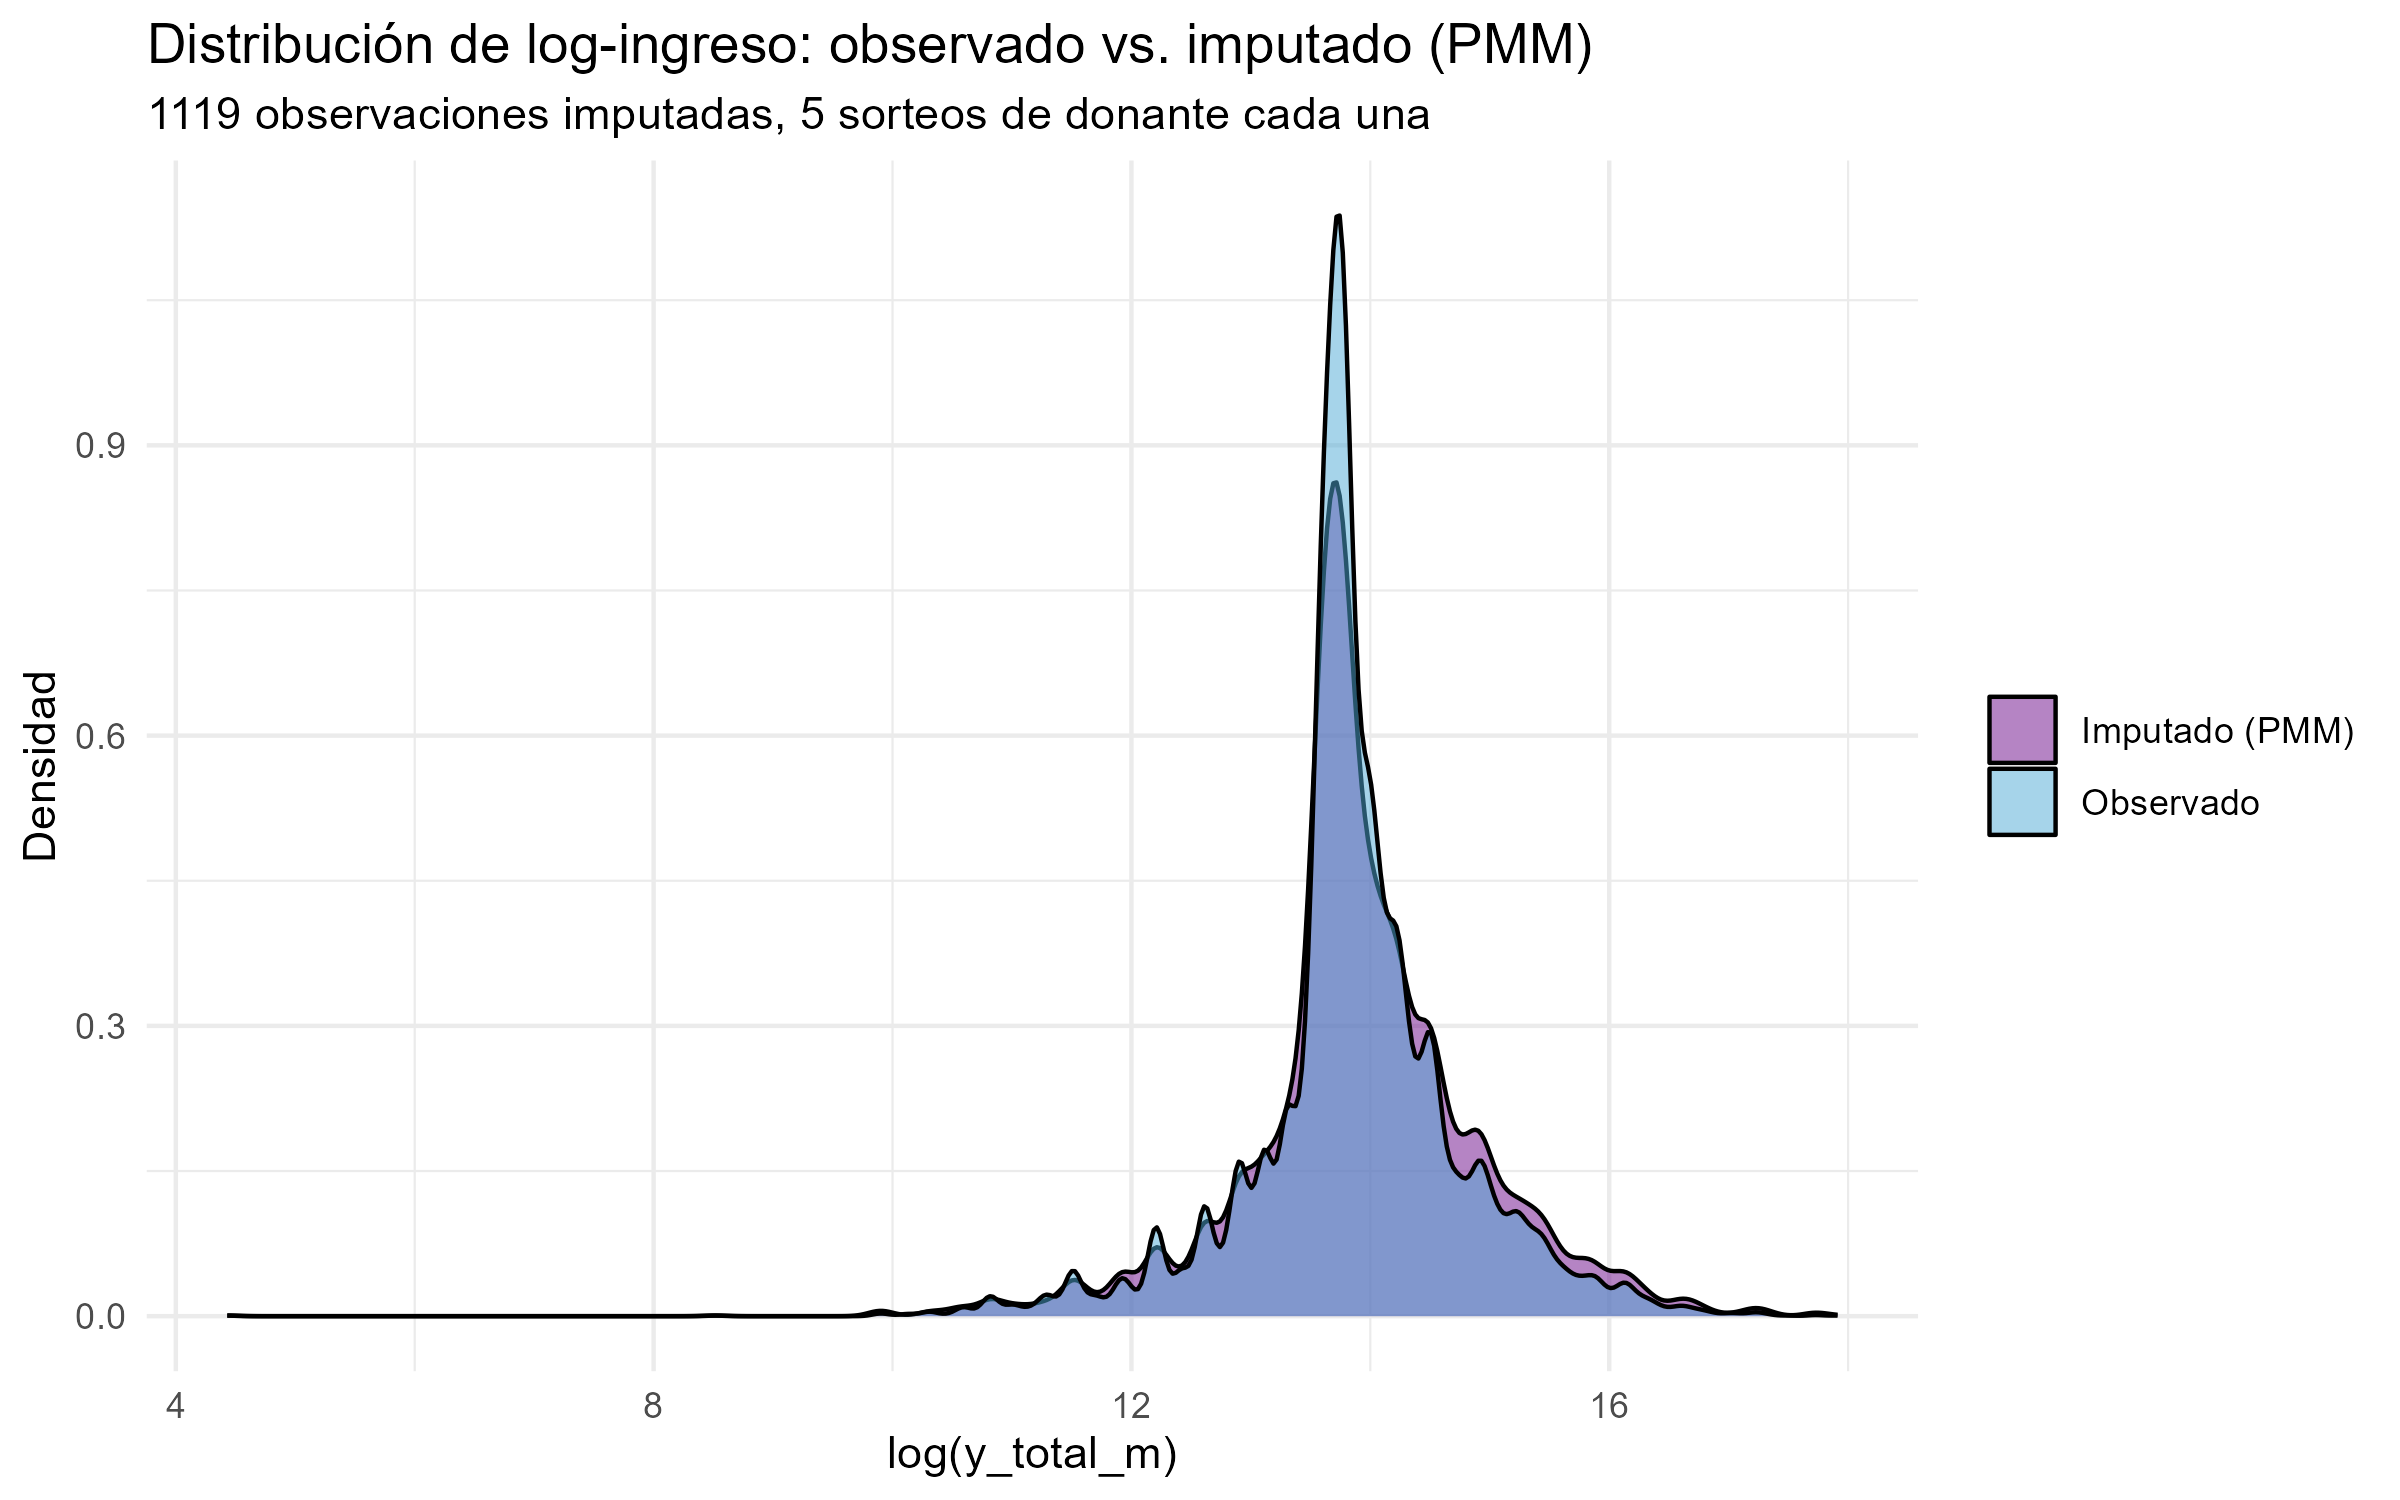
\includegraphics[width=\textwidth]{../../output/figures/section3_imputation_density.png}
      {\footnotesize Los valores imputados (PMM) se superponen bien con los
      observados: sin masa en valores implausibles.}
    \end{column}
    \begin{column}{0.48\textwidth}
      \centering
      \resizebox{\linewidth}{!}{
\begin{tabular}[t]{lrr}
\toprule
Model & RMSE (completos) & RMSE (imputado)\\
\midrule
Gender: HK + hours (05) & 0.745 & 0.745\\
Formal x firm size x college & 0.745 & 0.745\\
Género x nivel educativo & 0.776 & 0.776\\
Subsidio familiar x college & 0.779 & 0.779\\
Gender: HK controls (05) & 0.779 & 0.779\\
\addlinespace
Horas\textasciicircum{}2 x transferencias & 0.809 & 0.809\\
Age: conditional (04) & 0.812 & 0.812\\
Cuenta propia x college & 0.841 & 0.841\\
Age: unconditional (04) & 0.892 & 0.892\\
Gender: unconditional (05) & 0.907 & 0.907\\
\bottomrule
\end{tabular}
}
      \vspace{0.4em}
      {\footnotesize RMSE de validación casi idéntico entre regímenes: la
      imputación amplía el entrenamiento sin cambiar contra qué se valida
      (siempre ingreso \emph{real}). El ranking de modelos no cambia.}
    \end{column}
  \end{columns}
\end{frame}

% ---------------------------------------------------------------------------
\begin{frame}{Conclusiones}
  \begin{itemize}
    \item El mejor modelo de predicción (\PredBestModel) viene de la
      Sección 2, no de nuestras cinco especificaciones nuevas --- pero una de
      ellas (\PredSecondModel) iguala su desempeño, apoyada en una hipótesis
      económica distinta (prima de formalidad/tamaño de firma).
    \item RMSE de validación, LOOCV y AIC/BIC coinciden en el ranking: la
      comparación es robusta al criterio elegido.
    \item El sesgo de selección del ingreso faltante --- documentado desde la
      limpieza de datos --- \textbf{no distorsiona} materialmente el ranking
      ni el RMSE: imputar vía PMM deja los resultados prácticamente
      inalterados.
    \item Limitación real: el ejercicio sigue sin predecir el ingreso de
      trabajadores familiares sin remuneración (\texttt{relab} 6--7), que por
      definición no tienen salario monetario que imputar.
  \end{itemize}
\end{frame}

\end{document}
